\documentclass[a4paper,12pt]{report}
\usepackage[T2A]{fontenc}
\usepackage[utf8]{inputenc}
\usepackage[english,russian]{babel}
\usepackage{graphicx}
\usepackage{wrapfig}
\usepackage{mathtext} 				% русские буквы в фомулах
\usepackage{amsmath,amsfonts,amssymb,amsthm,mathtools} % AMS
\usepackage{icomma} % "Умная" запятая: $0,2$ --- число, $0, 2$ --- перечисление
\usepackage{capt-of}
\usepackage{appendix}
\usepackage{multirow}
\usepackage{hyperref}
\usepackage{floatrow}
\usepackage[left=2cm,right=2cm,
    top=2cm,bottom=2cm,bindingoffset=0cm]{geometry}
\usepackage{multicol} % Несколько колонок
\usepackage{gensymb}
\title{Отчёт по лабораторной работе №3

Определение ширины запрещенной зоны полупроводников по спектральной зависимости собственной проводимости}
\author{Плюскова Наталия}
\date{\today}

\begin{document}

\maketitle


\section*{1. Теоретические данные}

При воздействии на полупроводник излучения с энергией кванта $h\nu$, превышающей ширину запрещённой зоны $E_g$ в зоне проводимости, и соотвественно в валентной зоне возникают неравновесные электроны и дырки. Их появление связано с переходами электронов из валентной зоны проводимости. В результате увеличивается проводимость кристалла. Это явление называется собственной фотопроводимостью.

    В непрямозонных полупроводниках типа германия и кремния минимум зоны проводимости и максимум валентной зоны расположены в различных точках зоны Бриллюэна. В этом случае оптический переход электрона из вершины валентной зоны в минимум зоны проводимости возможен лишь при участии третьей частицы – фонона. В соответствии с законом сохранения импульса квазиимпульс такого фонона $q_{\text{ф}}\approx\hbar k_{\text{Б}}$, а энергия $\hbar\omega$ должна удовлетворять закону сохранения энергии:
    \begin{equation}
        h\nu = E_g\pm \hbar\omega_q+\hbar^2(k_n-k_c)^2/2m_n+\hbar^2k_p^2/2m_p
    \end{equation}
    где $k_n$ и $k_p$ -- начальные волновые числа электрона и дырки, а $k_c$ -- конечное волновое число электрона.

    Таким образом, край основной полосы поглощения в полупроводниках типа кремния и германия определяется непрямыми оптическими переходами, сопровождающимися поглощением и испусканием фононов. При этом для разрешённых переходов, которые доминируют в полупроводниках такого типа, коэффициент поглощения:

    \begin{equation}
        K=C\left[\frac{(h\nu-E_g+\hbar\omega_q)^2}{\exp{\frac{\hbar\omega_q}{kT}}-1}+\frac{(h\nu-E_g-\hbar\omega_q)^2}{1-\exp{-\frac{\hbar\omega_q}{kT}}}\right]
    \end{equation}
    При больших энергиях квантов $h\nu>(E_g+\hbar\omega_q)$ начинают преобладать переходы с эмиссией фононов и зависимость $K^{1/2}$ от $h\nu$ должна аппроксимироваться прямой, пересекающей ось энергии в точке $h\nu_1=E_g+\hbar\omega_q$.

    При рассмотрении случая сильного поглощения излечения в образце (оптически толстый образец), то есть при $d/K<<1$, где $d$ -- толщина образца, скорость генерации электронно-дырочных пар экспоненциально уменьшается от поверхности вглубь образца:
    \begin{equation}
        g(x)\approx K(1-R)N_0\exp{-Kx}
    \end{equation}
    где $R$ -- коэффициент отражения света, а $N_0$ -- поток квантов на единицу поверхности.

    Неоднородная германия электронов и дырок в направлении освещения приводит к появлению диффузионно-дрейфовых потоков носителей заряда: быстро диффундирующие носители (электроны) опережают медленные (дырки), что приводит к возникновению электрического поля, ускоряющего медленные носители и замедляющего быстрые и к появлению дрейфовых составляющих потоков. При этом изменение проводимости $\Delta\Sigma$ существенным образом зависит от граничных условий на поверхности образца:
    \begin{equation}
        \Delta\Sigma\sim N_0\left(1+\frac{S}{D}\frac{1}{K}\right)
    \end{equation}
    где $S$ -- скорость поверхностной рекомбинации, $D$ -- коэффициент амбиполярной диффузии.
    
    \section*{2. Экспериментальная часть}
    Для изменения фотоответа полупроводника $\Delta\Sigma$ образец включается последовательно с нагрузочным сопротивлением и источником постоянного напряжения. При освещении проводимость образца возрастает, происходит перераспределение напряжение между образцом и нагрузкой. В результате падение напряжения $U$ на образце при малом относительном увеличении проводимости уменьшается на величину
    \begin{equation}
        \Delta U=\varepsilon\frac{R_H\cdot R_0^2}{(R_H+R_0)^2}\Delta\Sigma
        \label{eq:deltaU}
    \end{equation}
    где $\varepsilon$ -- постоянное напряжение, $R_H$ и $R_0$ -- сопротивление нагрузки и образца, $\Sigma$ -- проводимость.

    Для повышения чувствительности измерения обычно проводят при периодическом прерывании светового потока. При этом соотношение (\ref{eq:deltaU}) характеризует амплитуду отрицательных импульсов напряжения на концах образца. Для исследования интересующих нас зависимостей $\Delta\Sigma/N_0$ от энергии кванта $h\nu$ наряду с $\Delta U$ необходимо знать спектральное распределение интенсивности источника излучения $N_0(h\nu)$.
    \begin{figure}[!htb]
        \centering
        \includegraphics[width=0.6\linewidth]{exp_scheme.pdf}
        \caption{Схема экспериментальной установки. 1 -- осветитель, 2 -- блок питания осветителя, 3 -- линзы, 4 -- механический модулятор излучения, 5 -- монохроматор, 6 -- блок питания образца, 7 -- схема включения образца, 8 -- усилитель}
    \end{figure}
    
\section*{3. Результаты эксперимента и обработка данных}

\subsection*{3.1. Кремний}
    Включаем лампу накаливания и фокусируем излучение монохроматора на образец Si. Подаём постоянное смещение $U$ на образец от источника напряжения. Вращая барабан длин волн, снимаем зависимость сигнала фотопроводимости $U$ от длины волны излучения. С помощью градуировочной кривой переводим деления барабана в энергии кванта $E$. Получаем зависимость $\frac{U}{N}(E)$ (рис. \ref{Si}), после чего строим зависимость $\sqrt{\frac{U}{N}}(E)$(рис. \ref{Si_add}).
    
    \begin{figure}[H]
        \centering
        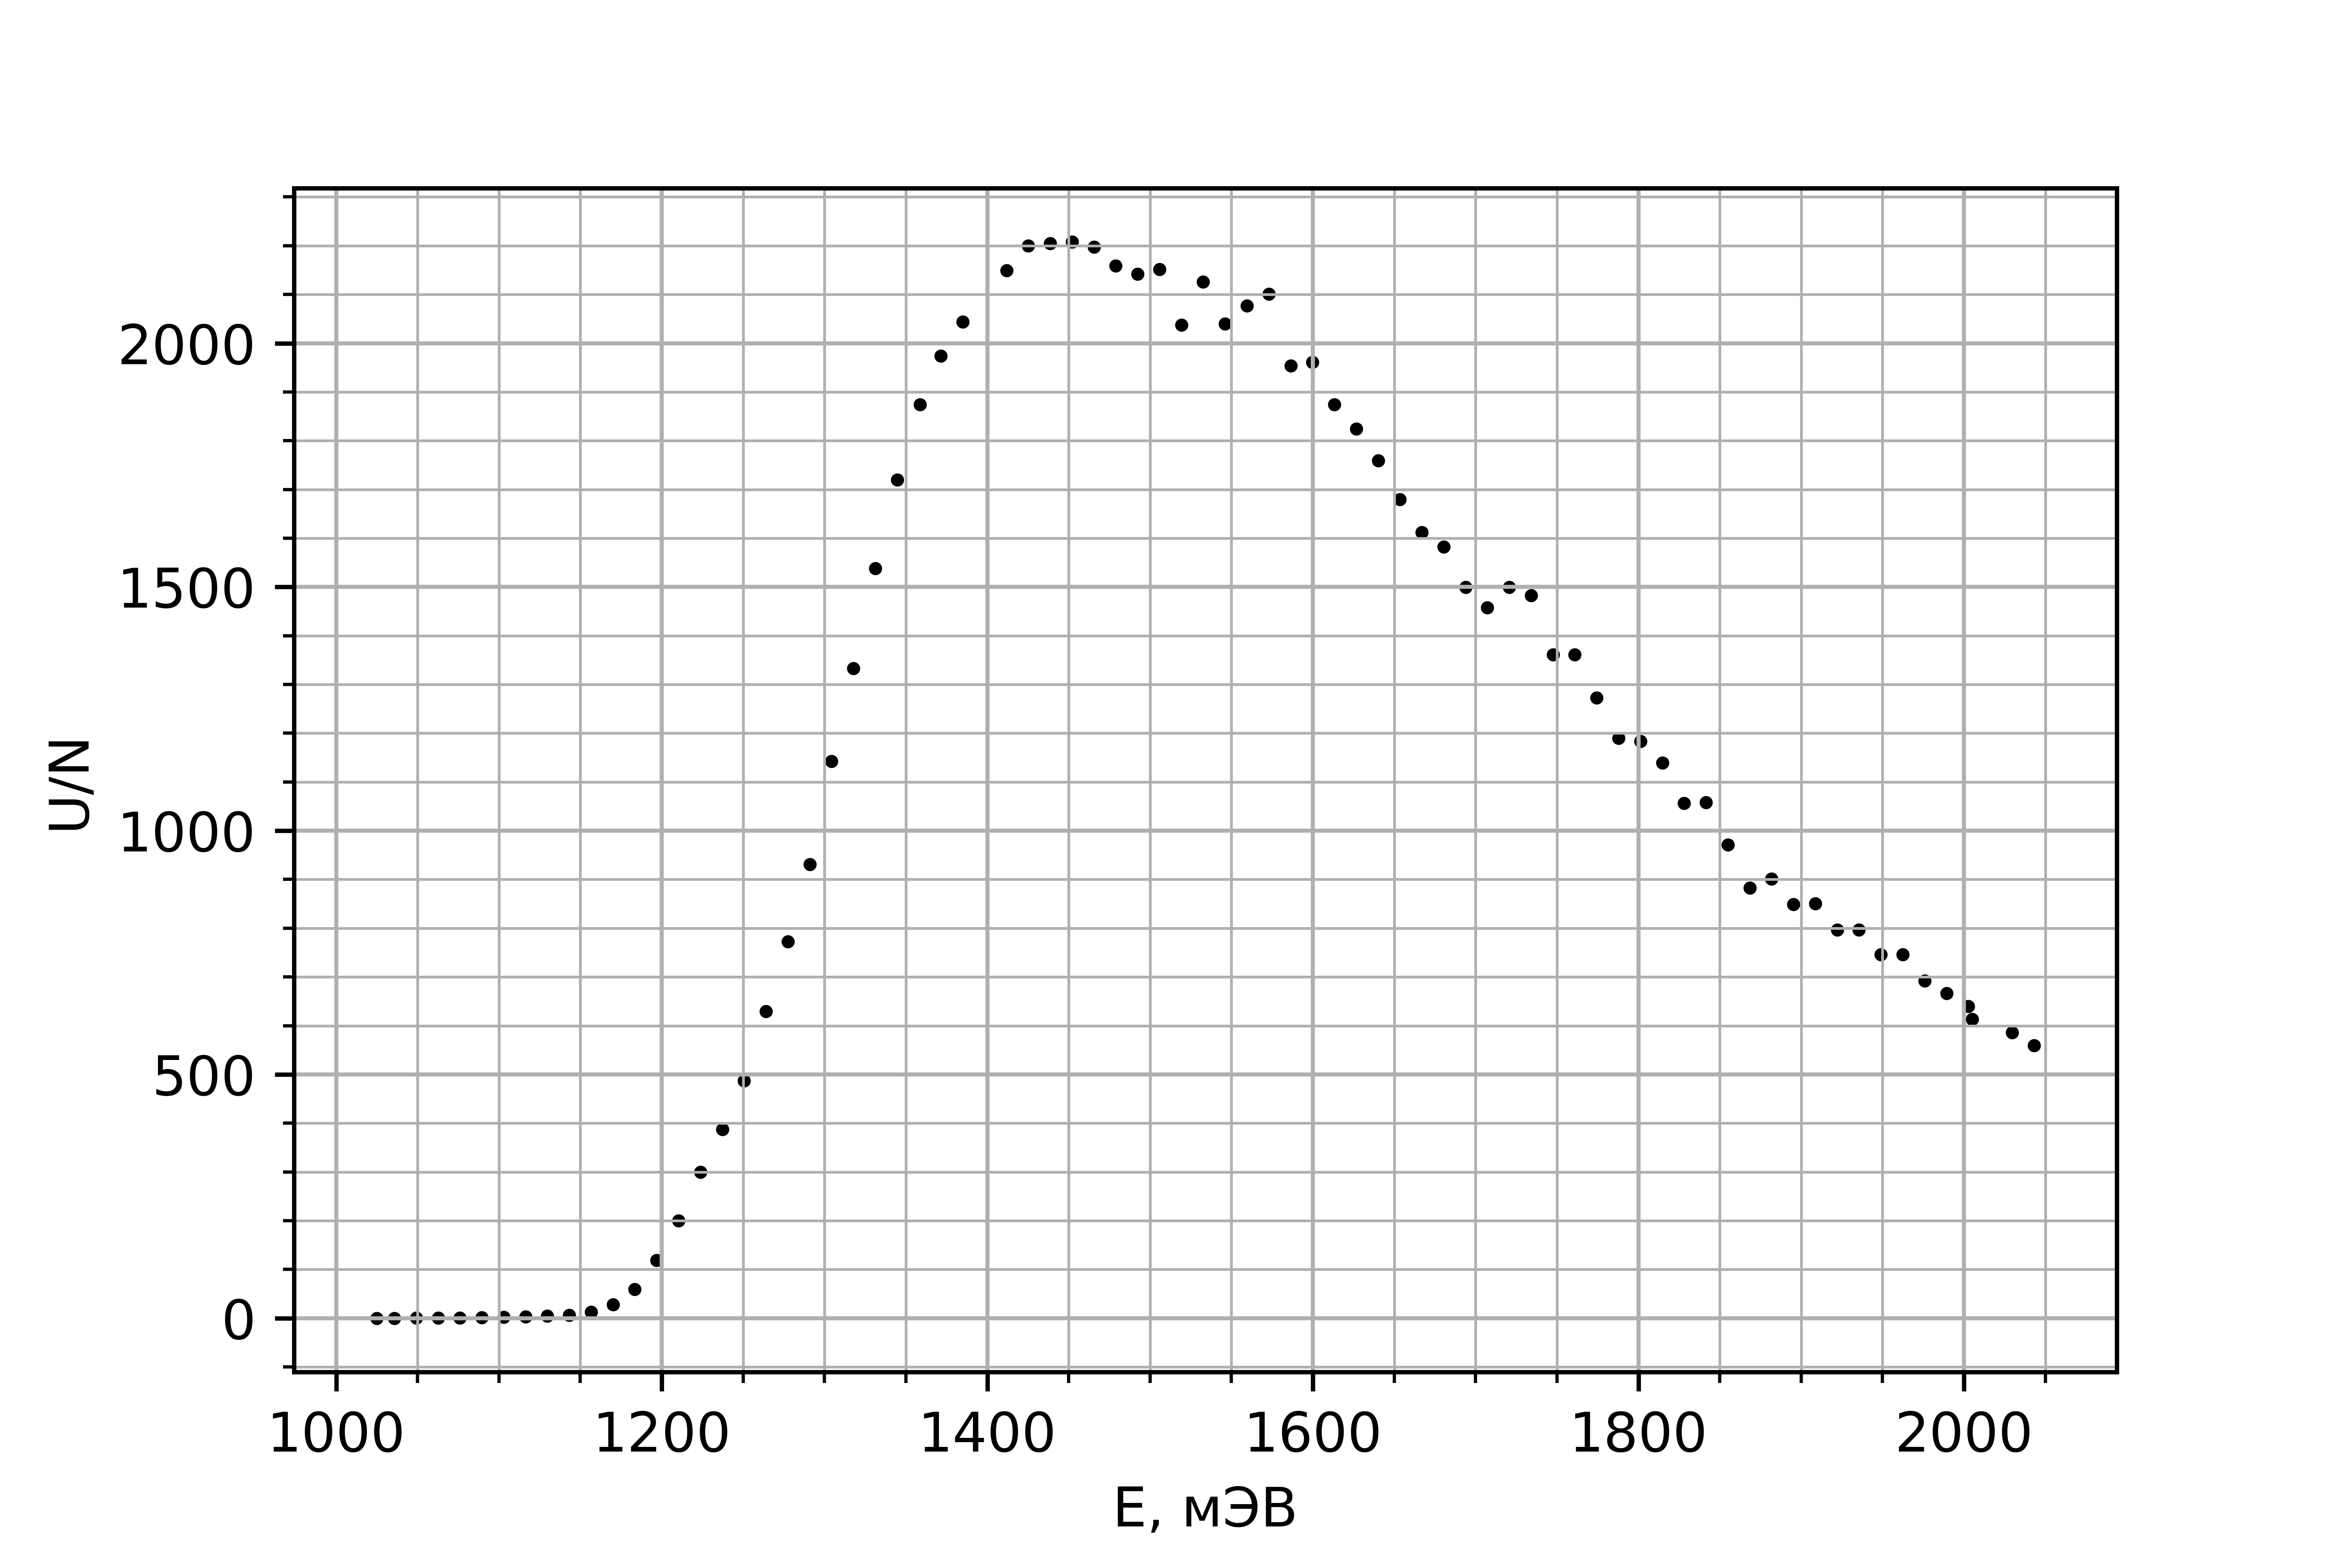
\includegraphics[width=0.6\linewidth]{Si.png}
        \caption{Зависимость $\frac{U}{N}(E)$} \label{Si}
    \end{figure}
    
    \begin{figure}[H]
        \centering
        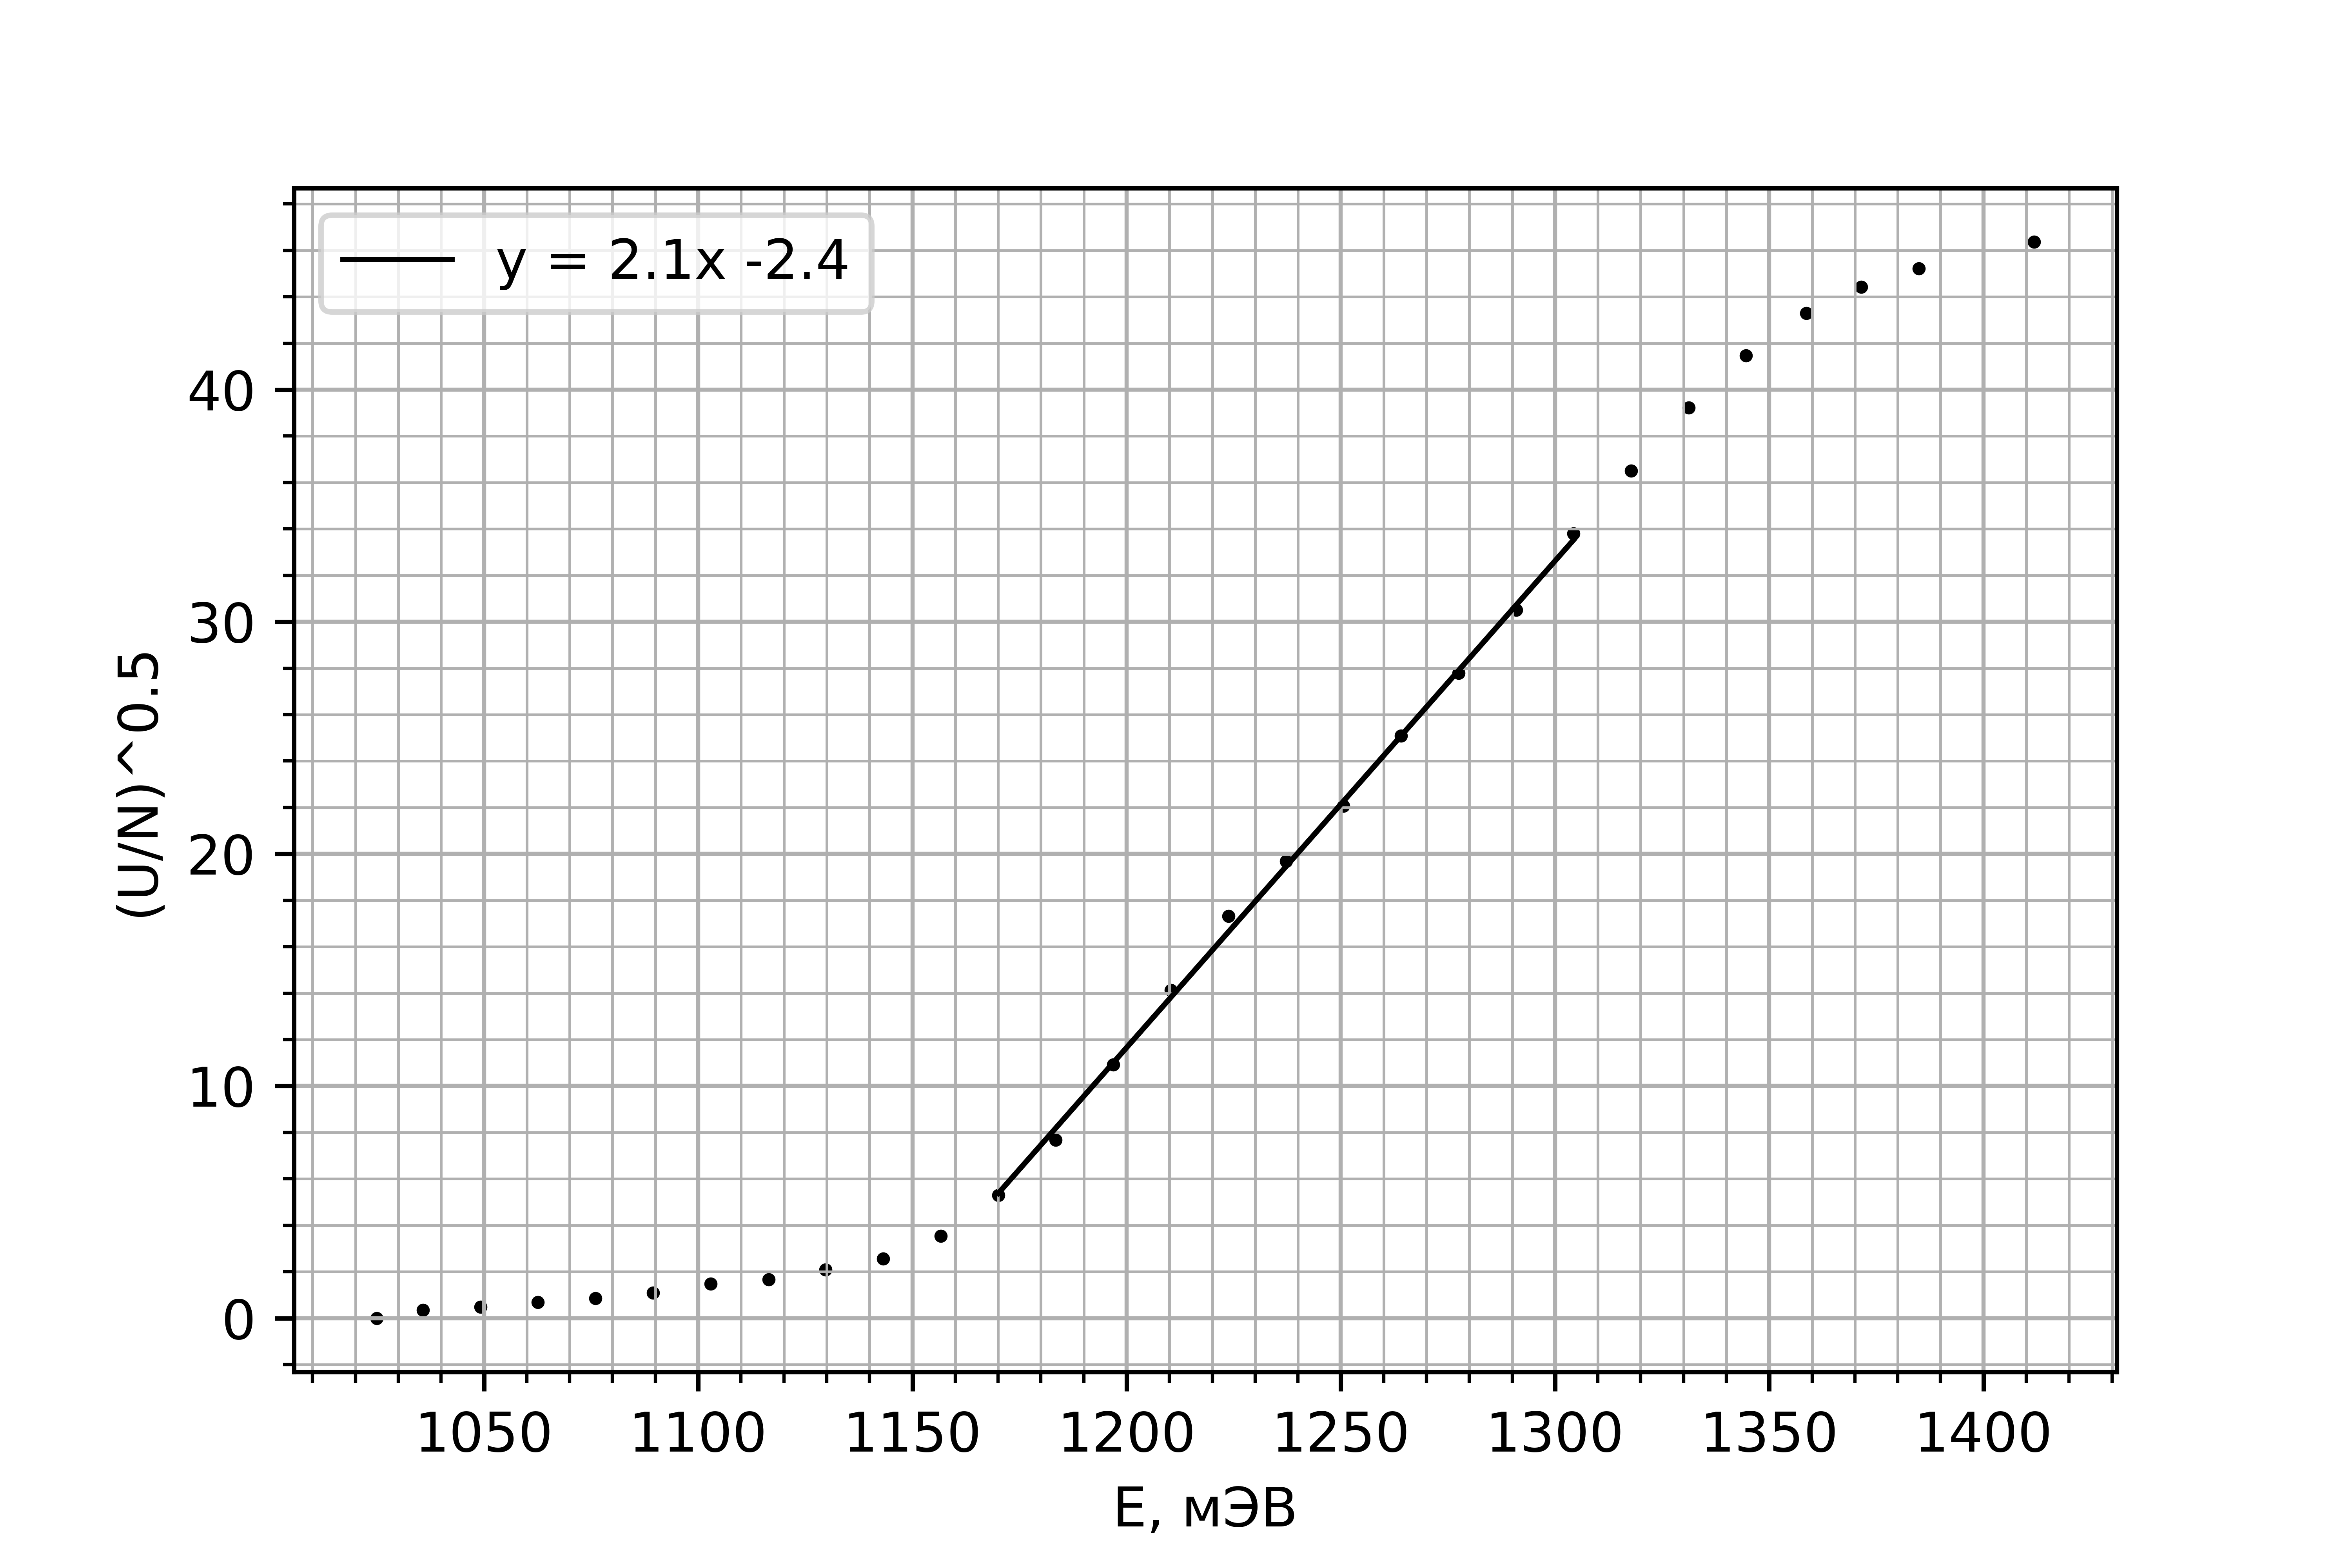
\includegraphics[width=0.6\linewidth]{Si_add.png}
        \caption{Зависимость $\sqrt{\frac{U}{N}}(E)$} \label{Si_add}
    \end{figure}

    Аппроксимируя линейный участок графика до оси энергии, получаем величину $E_g+\hbar\omega_{ph}$ как точку пересечения прямой с осью. Учитывая энергию фонона $\hbar\omega_{ph}=50$ мэВ, находим ширину запрещённой зоны кремния $E_g=1094.41$ мэВ.
    
    \subsection*{3.1 Селенид кадмия}
   Аналогично для образца CdSe. Получаем зависимость $\frac{U}{N}(E)$(рис. \ref{CdSe}), после чего строим график зависимости $(\frac{U}{N})^2(E)$(рис. \ref{CdSe_add}).
    \begin{figure}[H]
        \centering
        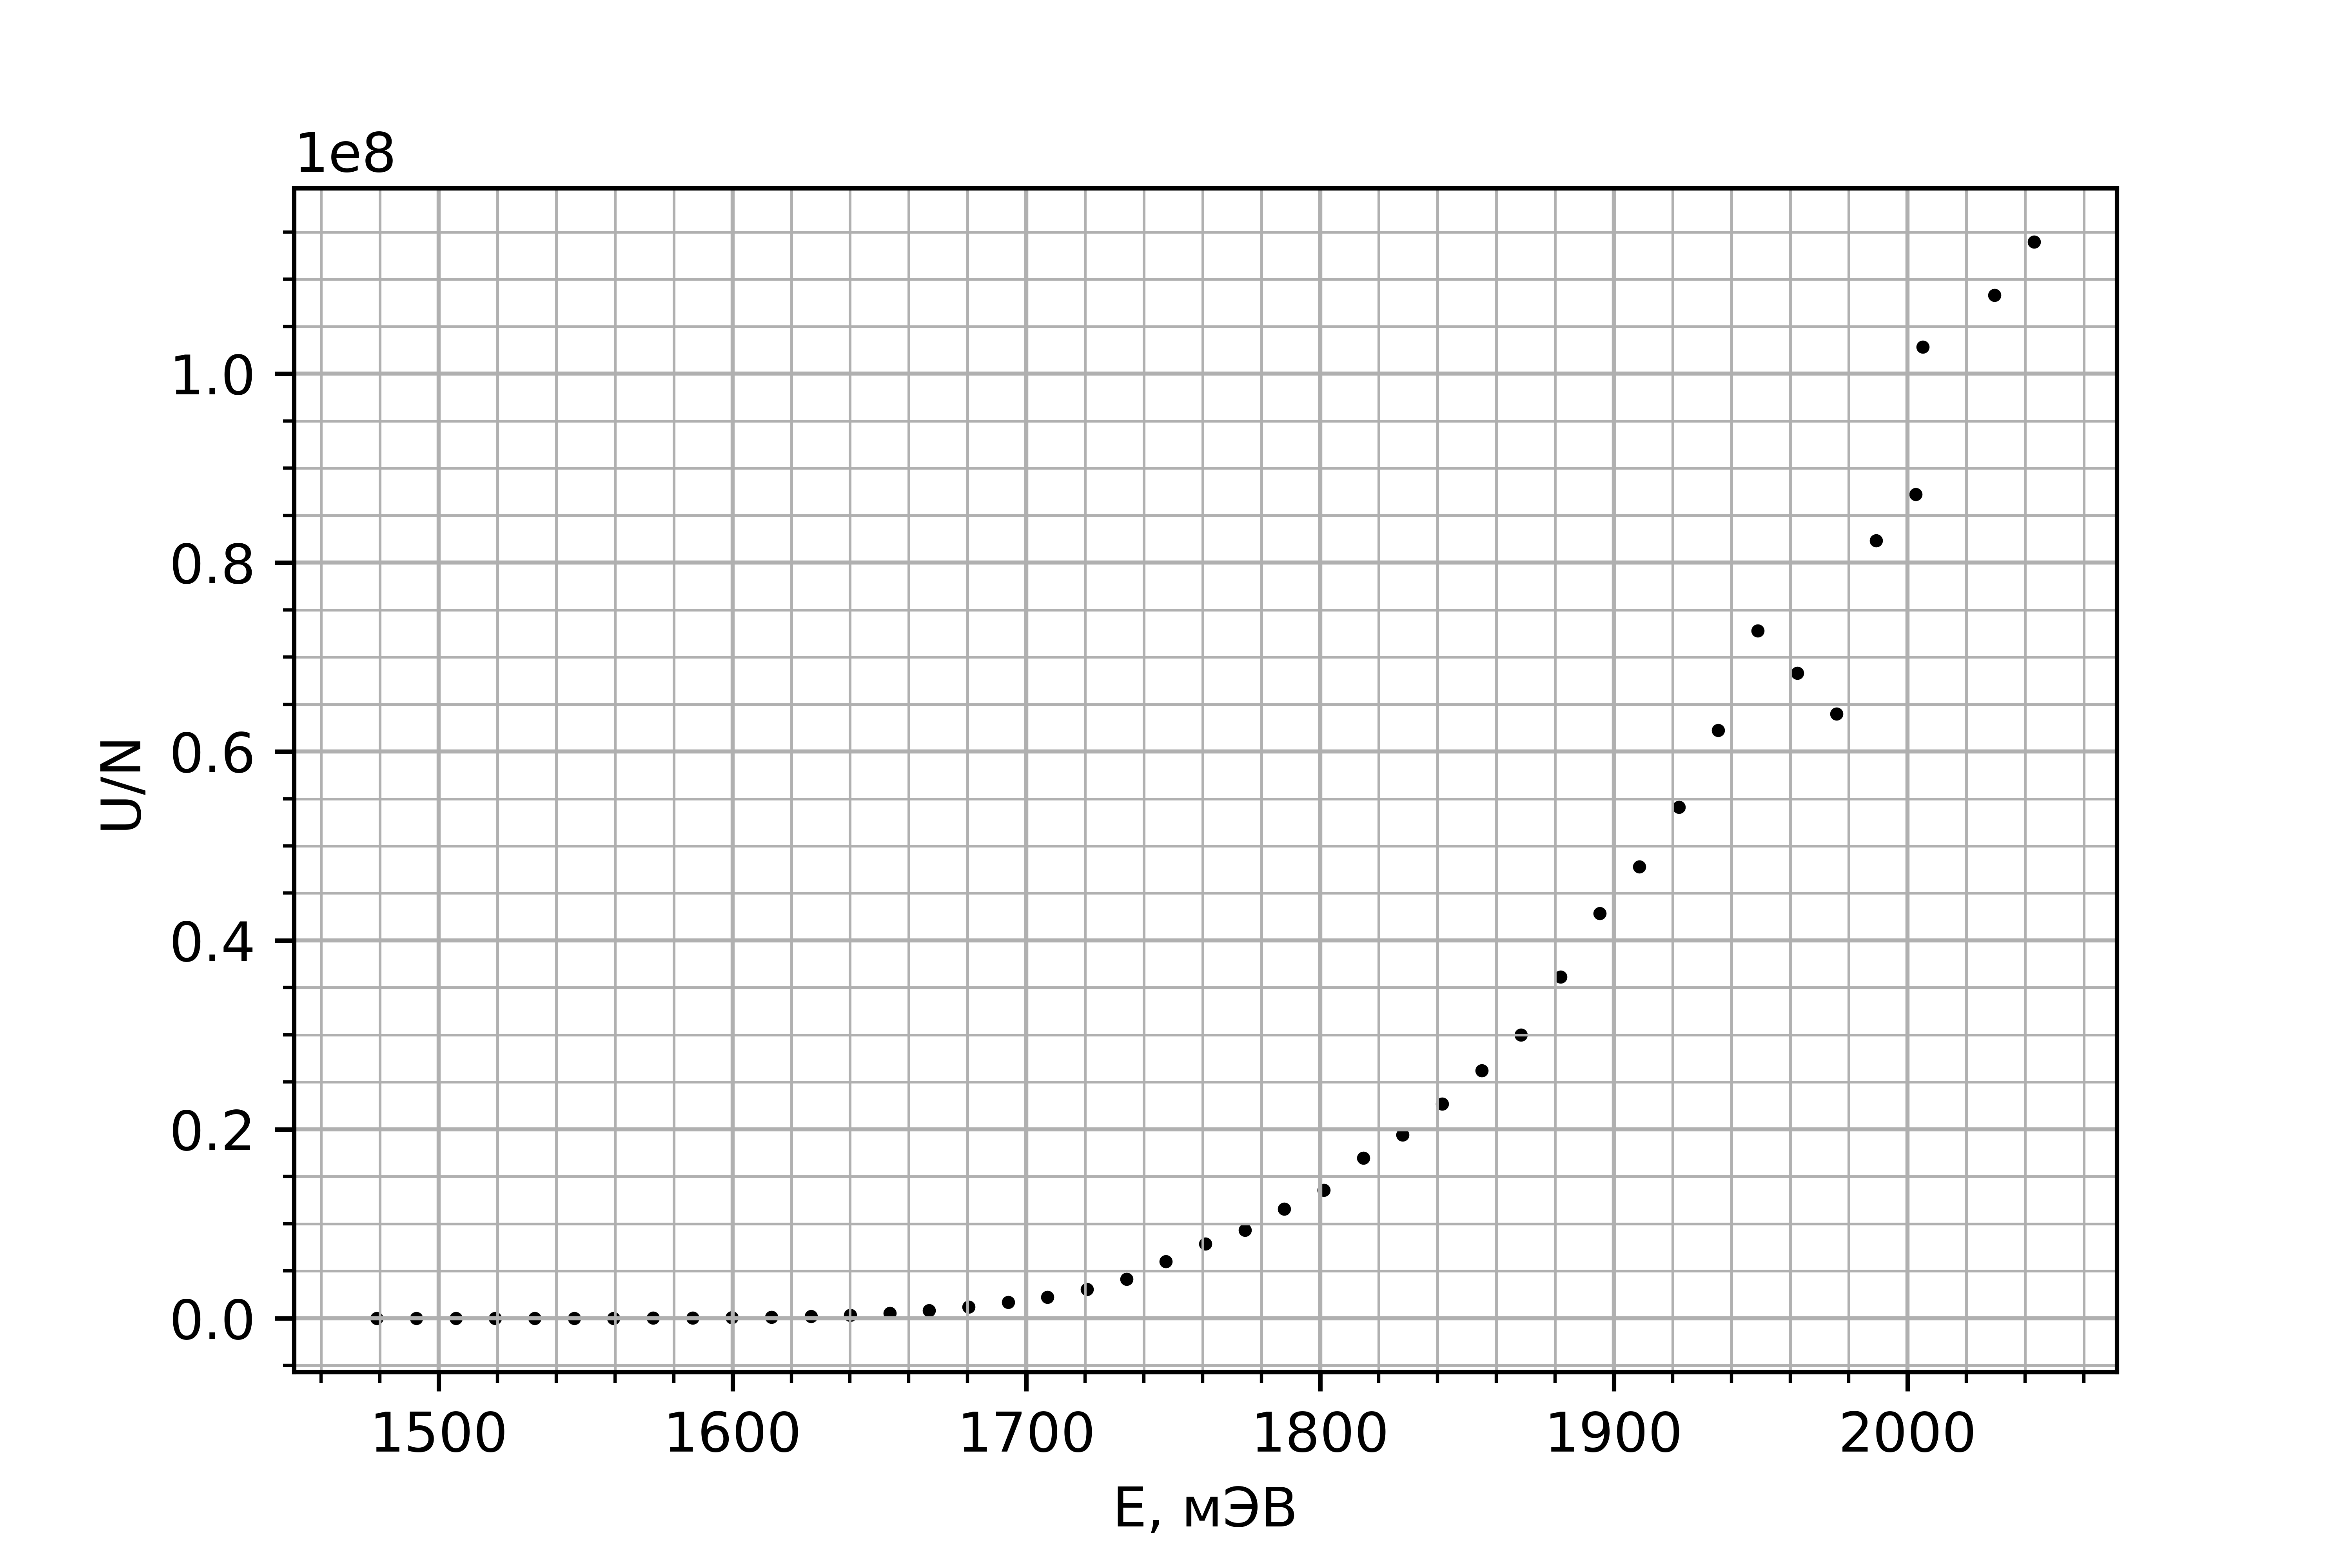
\includegraphics[width=0.6\linewidth]{CdSe.png}
        \caption{Зависимость $\frac{U}{N}(E)$} \label{CdSe}
    \end{figure}
    
    \begin{figure}[H]
        \centering
        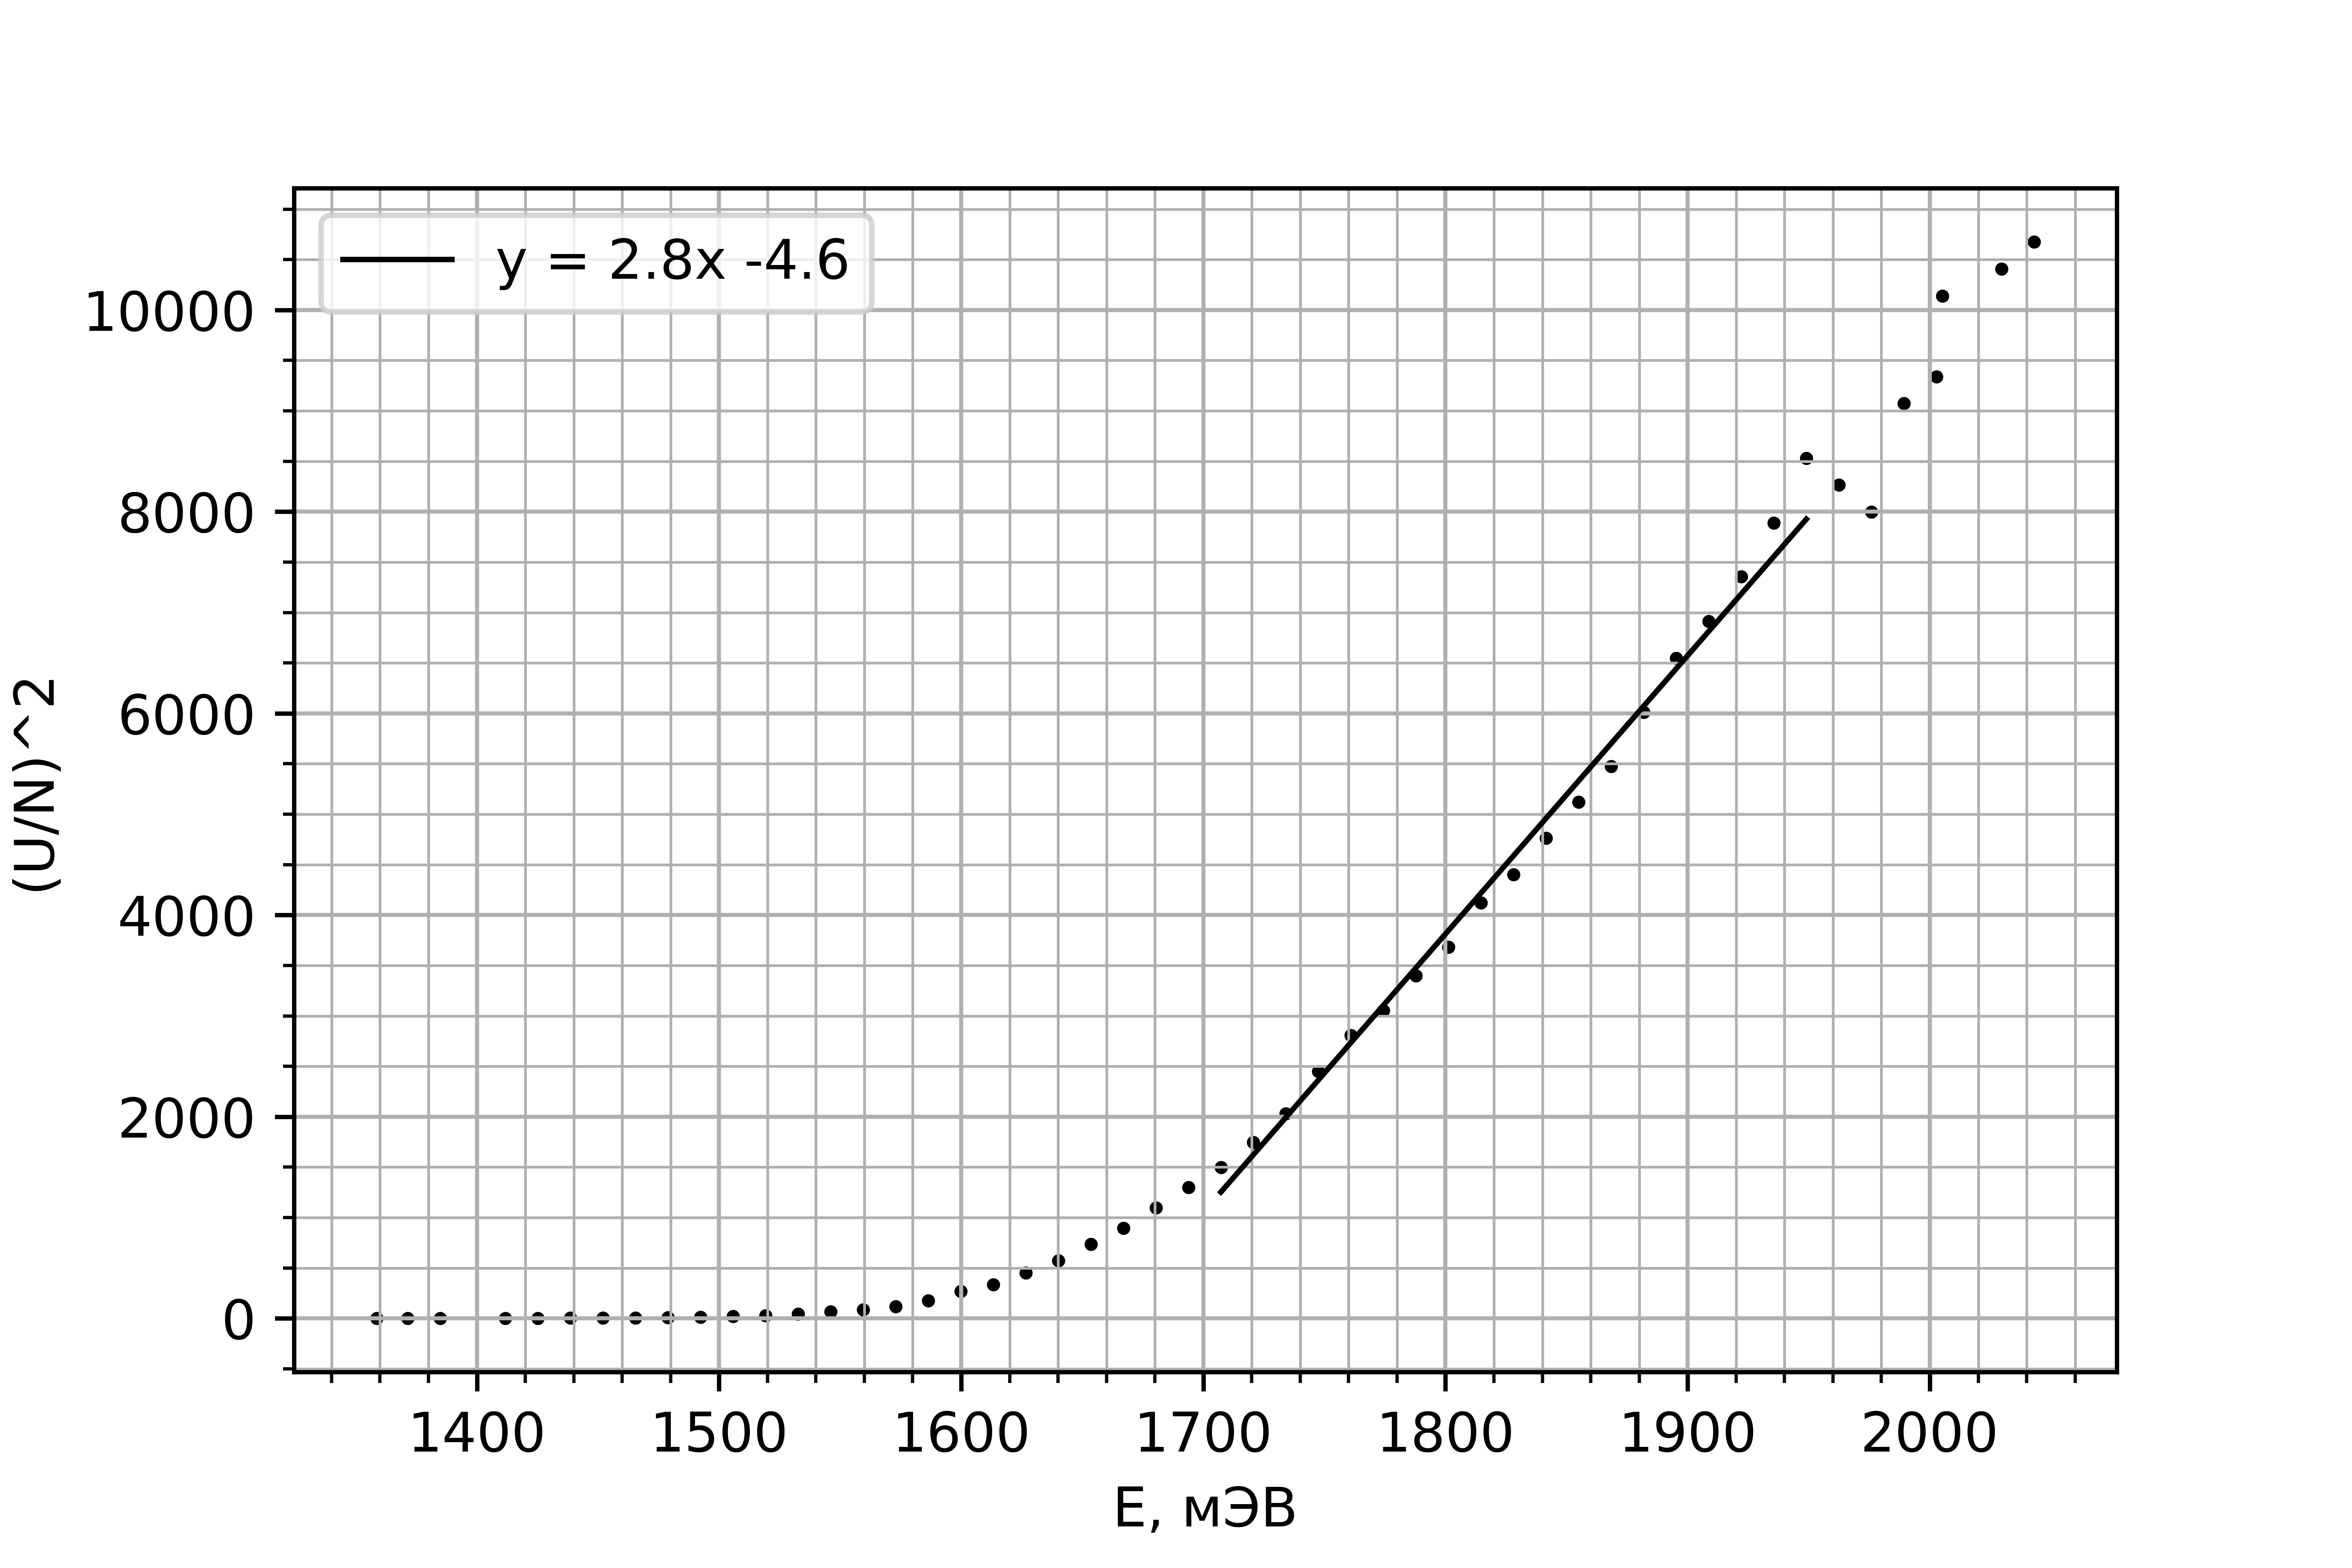
\includegraphics[width=0.6\linewidth]{CdSe_add.png}
        \caption{Зависимость $\sqrt{\frac{U}{N}}(E)$} \label{CdSe_add}
    \end{figure}

    Аппроксимируя линейный участок графика до оси энергии, получаем величину $E_g+\hbar\omega_{ph}$ как точку пересечения прямой с осью. Учитывая энергию фонона $\hbar\omega_{ph}=50$ мэВ, находим ширину запрещённой зоны кремния $E_g=1661.84$ мэВ.
    \section*{4. Выводы}
    \begin{enumerate}
        \item Изучили принципы собственной фотопроводимости в полупроводниках
        \item При проведении работы нашли ширину запрещённой зоны кремния и селенида кадмия: 1094.41 мэВ и 1661.84 мэВ соотвественно.
    \end{enumerate}
\section*{5. Приложение}

    \begin{figure}[H]
        \centering
        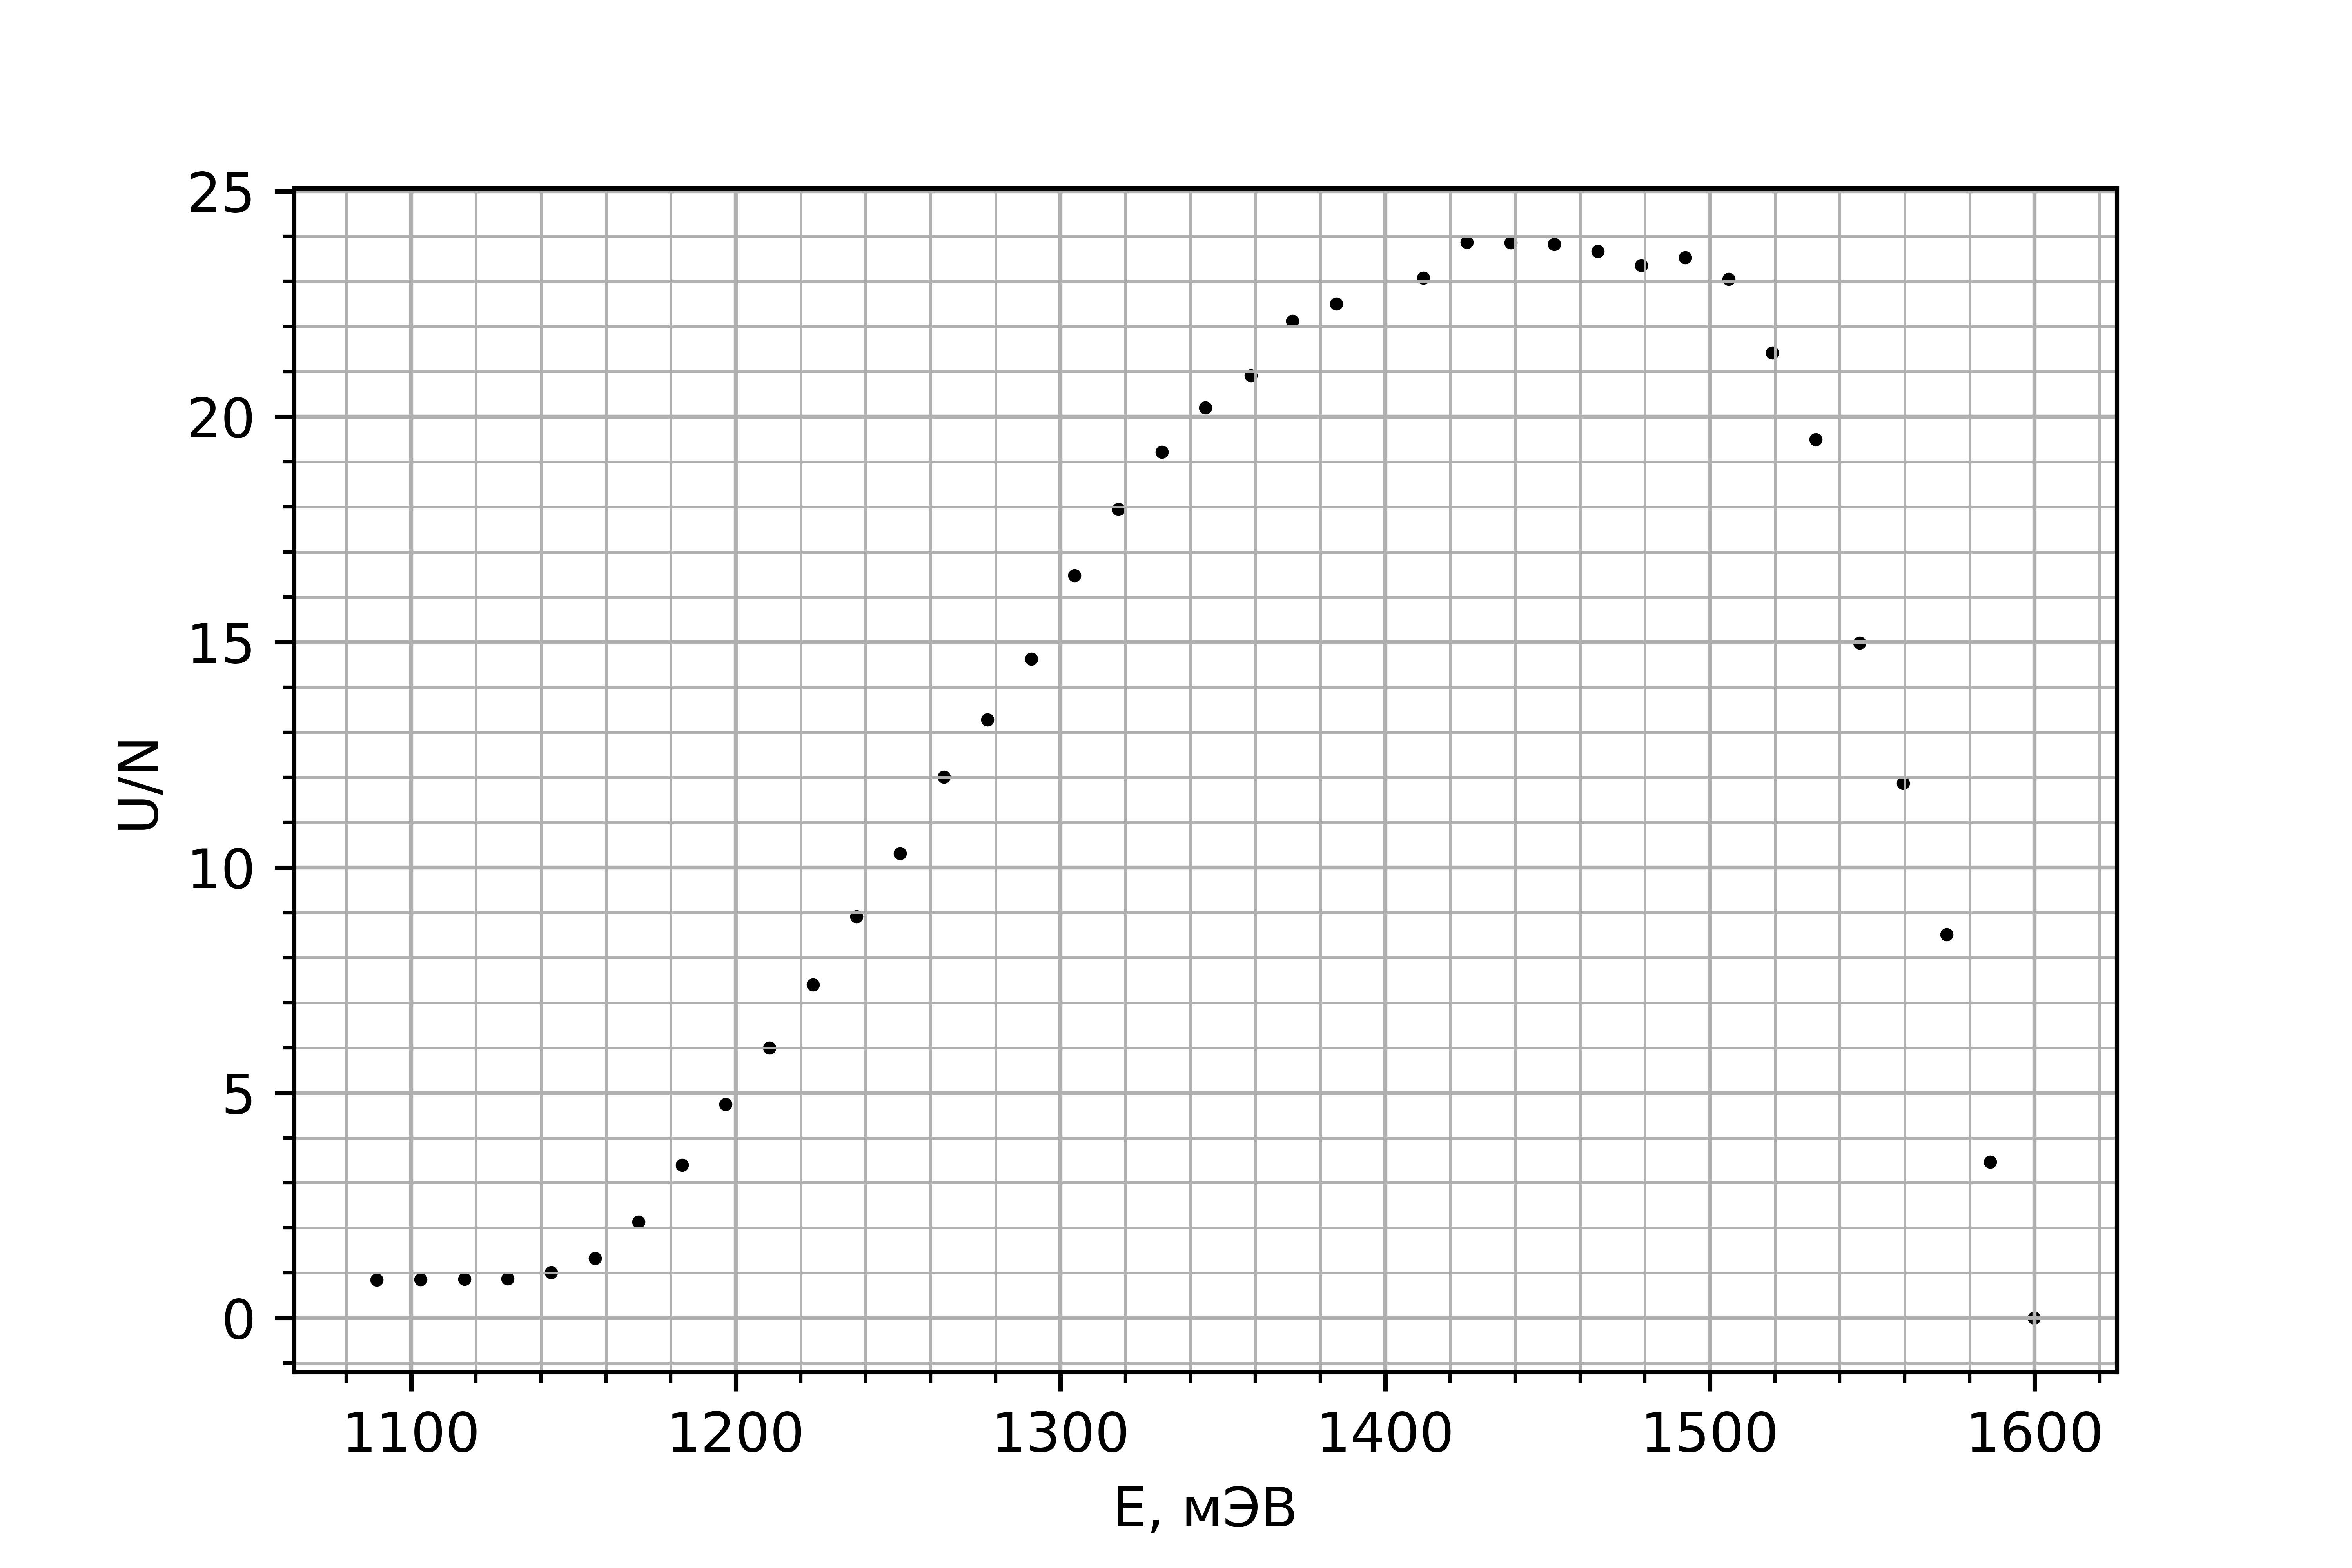
\includegraphics[width=0.6\linewidth]{Si+GaAs.png}
        \caption{Зависимость $\sqrt{\frac{U}{N}}(E)$ для кремниевого образца с кремниевым фильтром}
    \end{figure}

\newpage
\section*{6. Вопросы}

\begin{enumerate}
    \item Что такое скорость оптической генерации? Её размерность? \par 
    Cкоростью оптической генерации называют количество пар электронов и дырок, появляющихся в единице объёма за единицу времени. Таким образом размерность скорости оптической генерации – $[g] = c^{-1} \cdot м^{-3}$.

    \item Разъяснить понятие «оптически тонкий образец» \par 
    В случае, когда скорость оптической генерации слабо изменяется в направлении освещения, говорят, что образец является оптически тонким. Это утверждение аналогично тому, что поглощение света в образце очень слабое. Математическое утверждение выглядит следующим образом:
    $g \sim e^{-Kx}$ , где К – коэффициент поглощения. Отсюда следует, что образец называется оптически тонким при выполнении условия $Kd \ll 1$ 

    \item  Получить выражение для скорости оптической генерации в случае, когда образец можно считать оптически тонким. \par 
    $$g(x) = \beta \frac{KN_0 (1-R)}{1 - R^2 e^{-2Kd}} (e^{-Kx} + Re^{-K(2d-x)})$$
    При малой оптической толщине $kd<<1$. Для $\beta \approxeq 1$
    $$g(x) \approxeq \frac{KN_0(1-R)}{1-R^2(1-2Kd)} ((1-Kx) + R(1-2Kd + Kx))$$
    $$g(x) \approxeq \frac{KN_0 (1-R)}{(1-R)^2} (1+R) = KN_0$$

    \item Как зависит фотопроводимость от коэффициента поглощения при энергиях света, когда образец можно считать оптически тонким? Оптически толстым? \par
    \begin{enumerate}
        \item Опт. тонкий \par 
        Из $\Delta n = \Delta p$ - условие электронейтральности вытекает $\tau_n = \tau_p = \tau$:
        $$\Delta \Sigma = \frac{e(\mu_n + \mu_p) \omega}{l} K(h\nu) N_0 \tau$$
        $$\Delta \Sigma \sim KN_0\tau$$

        \item Опт. толстый \par 
        При $g \approxeq K(1-R)N_0 e^{-Kx}$
        $$\Delta \Sigma \sim \frac{N_0}{\tau}$$
    \end{enumerate}

    \item Рассчитать коэффициент пропорциональности между энергией кванта света в эВ и соответствующей длиной волны в мкм.\par 
    $E = h \nu = h \frac{c}{\lambda} \longrightarrow \lambda E = hc = const \Longrightarrow$ 1 эВ $\Leftrightarrow$ 1.240 мкм.

    \item Ширина зоны прямозонного полупроводника 0,8 эВ. При какой длине волны (в мкм) на фоторезисторе из такого материала можно наблюдать собственную  фотопроводимость? \par 
    $\lambda E = hc = 1.240$ (мкм эВ) $\longrightarrow$ $\lambda = 1.5$ мкм

    \item Темновое сопротивление фоторезистора составляет 40 кОм. Как и какое нагрузочное сопротивление надо припаять в схему для регистрации фотопроводимости, чтобы получить максимальный сигнал? \par 
    $$\Delta u = \varepsilon \frac{R_n R_o}{(R_n + R_o)} \frac{\Delta \Sigma}{\Sigma_o}$$
    $$\Delta u = \varepsilon \frac{R_o^2}{(R_n + R_o)^2} \Delta \Sigma R_n \rightarrow \frac{\partial \Delta u}{\partial R_n} = 0$$
    $$R_n = R_o = 40\; k\Omega$$

    \item На какое расстояние успеют продиффудировать избыточные электроны в Si, если время жизни носителей составляет 10-4 с? \par 
    

    \item На рис.\ref{9} показаны спектральные зависимости фотопроводимости CdS  и CdSe. Пунктирные и сплошные линии соответствуют разным температурам. Какие линии  каким температурам соответствуют? \par 
    \begin{figure}[H]
        \centering
        \includegraphics[scale = 0.6]{9.png}
        \caption{}
        \label{9}
    \end{figure} 

    \item Нарисуйте качественно зависимость сигнала фотопроводимости кремниевого фоторезистора от энергии кванта. Энергия фонона  50 мэВ. \par 

    \item Как зависит фотопроводимость U/N при Kd1 от $h \nu$ в прямозонных полупроводниках? \par 

    \item  На рис.\ref{12} приведены результаты измерения сигнала  U фотопроводимости (ФП) образца CdSe  в зависимости от энергии $h \nu$ падающего на образец света. Этот ПП – прямозонный. \par 
    \begin{figure}[H]
        \centering
        \includegraphics[scale = 0.6]{12.png}
        \caption{}
        \label{12}
    \end{figure} 
    Из графика зависимости коэффициента полгощения от энергии фотонов для кремния $K(h \nu)$ видно изменение оптических свойств, соответсвующее переходу из оптически тонкого состояни я в оптически толстое ($kd \sim 1$). При $K \approxeq 110\; cm^{-1}$, те $d \approx 91$ мкм.
    \item Рассчитать удельное сопротивление кремния, данные в таблице в конце описания работы. 
    \item По спектрам поглощения (см методичку) показать область прямых и непрямых переходов в Si и Ge 

\end{enumerate}

\end{document}
